Due to our limitation in computing resources, we can only present our approaches for the first 30 bins (meaning videos with age ranging from 1 day to 30 days). For each bin, we create 5-fold cross-validation with 80\% of our data for training, and the other 20\% for testing. The average results over these are reported.

%We set the learning rate $\eta=1$, $\lambda=0.01$. The maximum of iteration is $maxIter=3$. We did try with other values of $maxIter$ up to 10, but they do not give significant gains and take more time to run.

\subsubsection{Classification Results}
	The accuracy and $F_1$-score of our logistic regression are presented in Table \ref{tbl:acc} and Table \ref{tbl:f1} correspondingly. For each metric, we present four approaches: original logistic regression (ORG), logistic regression with augmented features (AUG), logistic regression with weighed gradients (GRAD) and logistic regression with both extensions (BOTH). Each approach we compare with its corresponding ensemble version as described in section \ref{subsec:ext2}. 
	
	Although all the approaches return barely above 50\%, there are some observations. First, the extension with augmented features have better performance than original approach. Meanwhile, the weighted-gradient extension is actually less effective at prediction.  That makes senses since we put more weights on the gradients, and thus need much better control on the learning rate to avoid having parameters would oscillate between both side of the optimal values. It also explains why the 'BOTH' method performs the worst in accuracy and $F_1$-scores among the methods explored.
	
	\begin{table}[h]
	\caption{Average of Accuracy over 5 folds of 30 bins.}
	\label{tbl:acc}
		\begin{center}
			\begin{tabular}{| l | c | c |}						
			\hline
			Approach & Single Predictor & Ensemble \\ \hline
			BOTH & 0.513 & \textbf{0.526} \\ \hline
			GRAD & 0.514 & \textbf{0.527} \\ \hline
			AUG & 0.516 & \textbf{0.534} \\ \hline
			ORG & 0.514 & \textbf{0.532} \\ \hline		
			\end{tabular}
		\end{center}	
	\end{table}

	\begin{table}[h]
	\caption{Average of $F_1$-score over 5 folds of 30 bins.}
	\label{tbl:f1}
		\begin{center}		
			\begin{tabular}{| l | c | c |}
			\hline
				Approach & Single Predictor & Ensemble \\ \hline
				BOTH & \textbf{0.468} & 0.463 \\ \hline
				GRAD & \textbf{0.451} & 0.443 \\ \hline
				AUG & 0.473 & \textbf{0.503} \\ \hline
				ORG & 0.455 & \textbf{0.468} \\ \hline
			\end{tabular}
		\end{center}
	\end{table}

	Most of the ensemble methods have better performance (both in accuracy and $F_1$-scores) than single predictions. That supports our hypothesis that by partitioning the videos into bins, we worsen the sparseness in each bin's data. Hence by using an weighted combination of all classifiers, we can pass information between the bins to achieve better performance. Recall that the ensemble methods work only if all the individual predictors have good performance in their own data. Since 'BOTH' and 'GRAD' have lower accuracy in prediction, ensemble methods do not work when using them as basic classfiers. That explains the interesting observation that $F_1$-scores are better for single predictors in these cases.
	
\subsubsection{Regression Results}
	When evaluating our predictions directly, we found an RMSE of 0.93, indicating that we were on average off of the true value by just under an order of magnitude.  Without the context from the \textbf{0-1 loss function}, however, it is hard to say whether we should be impressed.
	
	The \textbf{0-1 loss function} allowed us to compare this method's results to those of the logistic regression method.  Our \textbf{0-1 loss function} results were not significantly any greater than 50\%.  While it is not surprising to us that linear regression performs more poorly than classification for the ranking problem, we are surprised that our accuracy is so comparable to that of random guessing, indicating that this technique yielded no measurable value for the ranking problem.
	
	A likely cause is that this problem may not be linear in nature -- in fact, it would admittedly be surprising if it were.  We tested our accuracy on the training data as well as on the testing data, and found that it performed just as poorly in each, indicating that the weak results on our testing data did not stem from over-fitting.
	
	In order to investigate further, we plotted our output against the true number of views (for a random subset of our data):

	\begin{figure}[!h]
		\begin{center}
			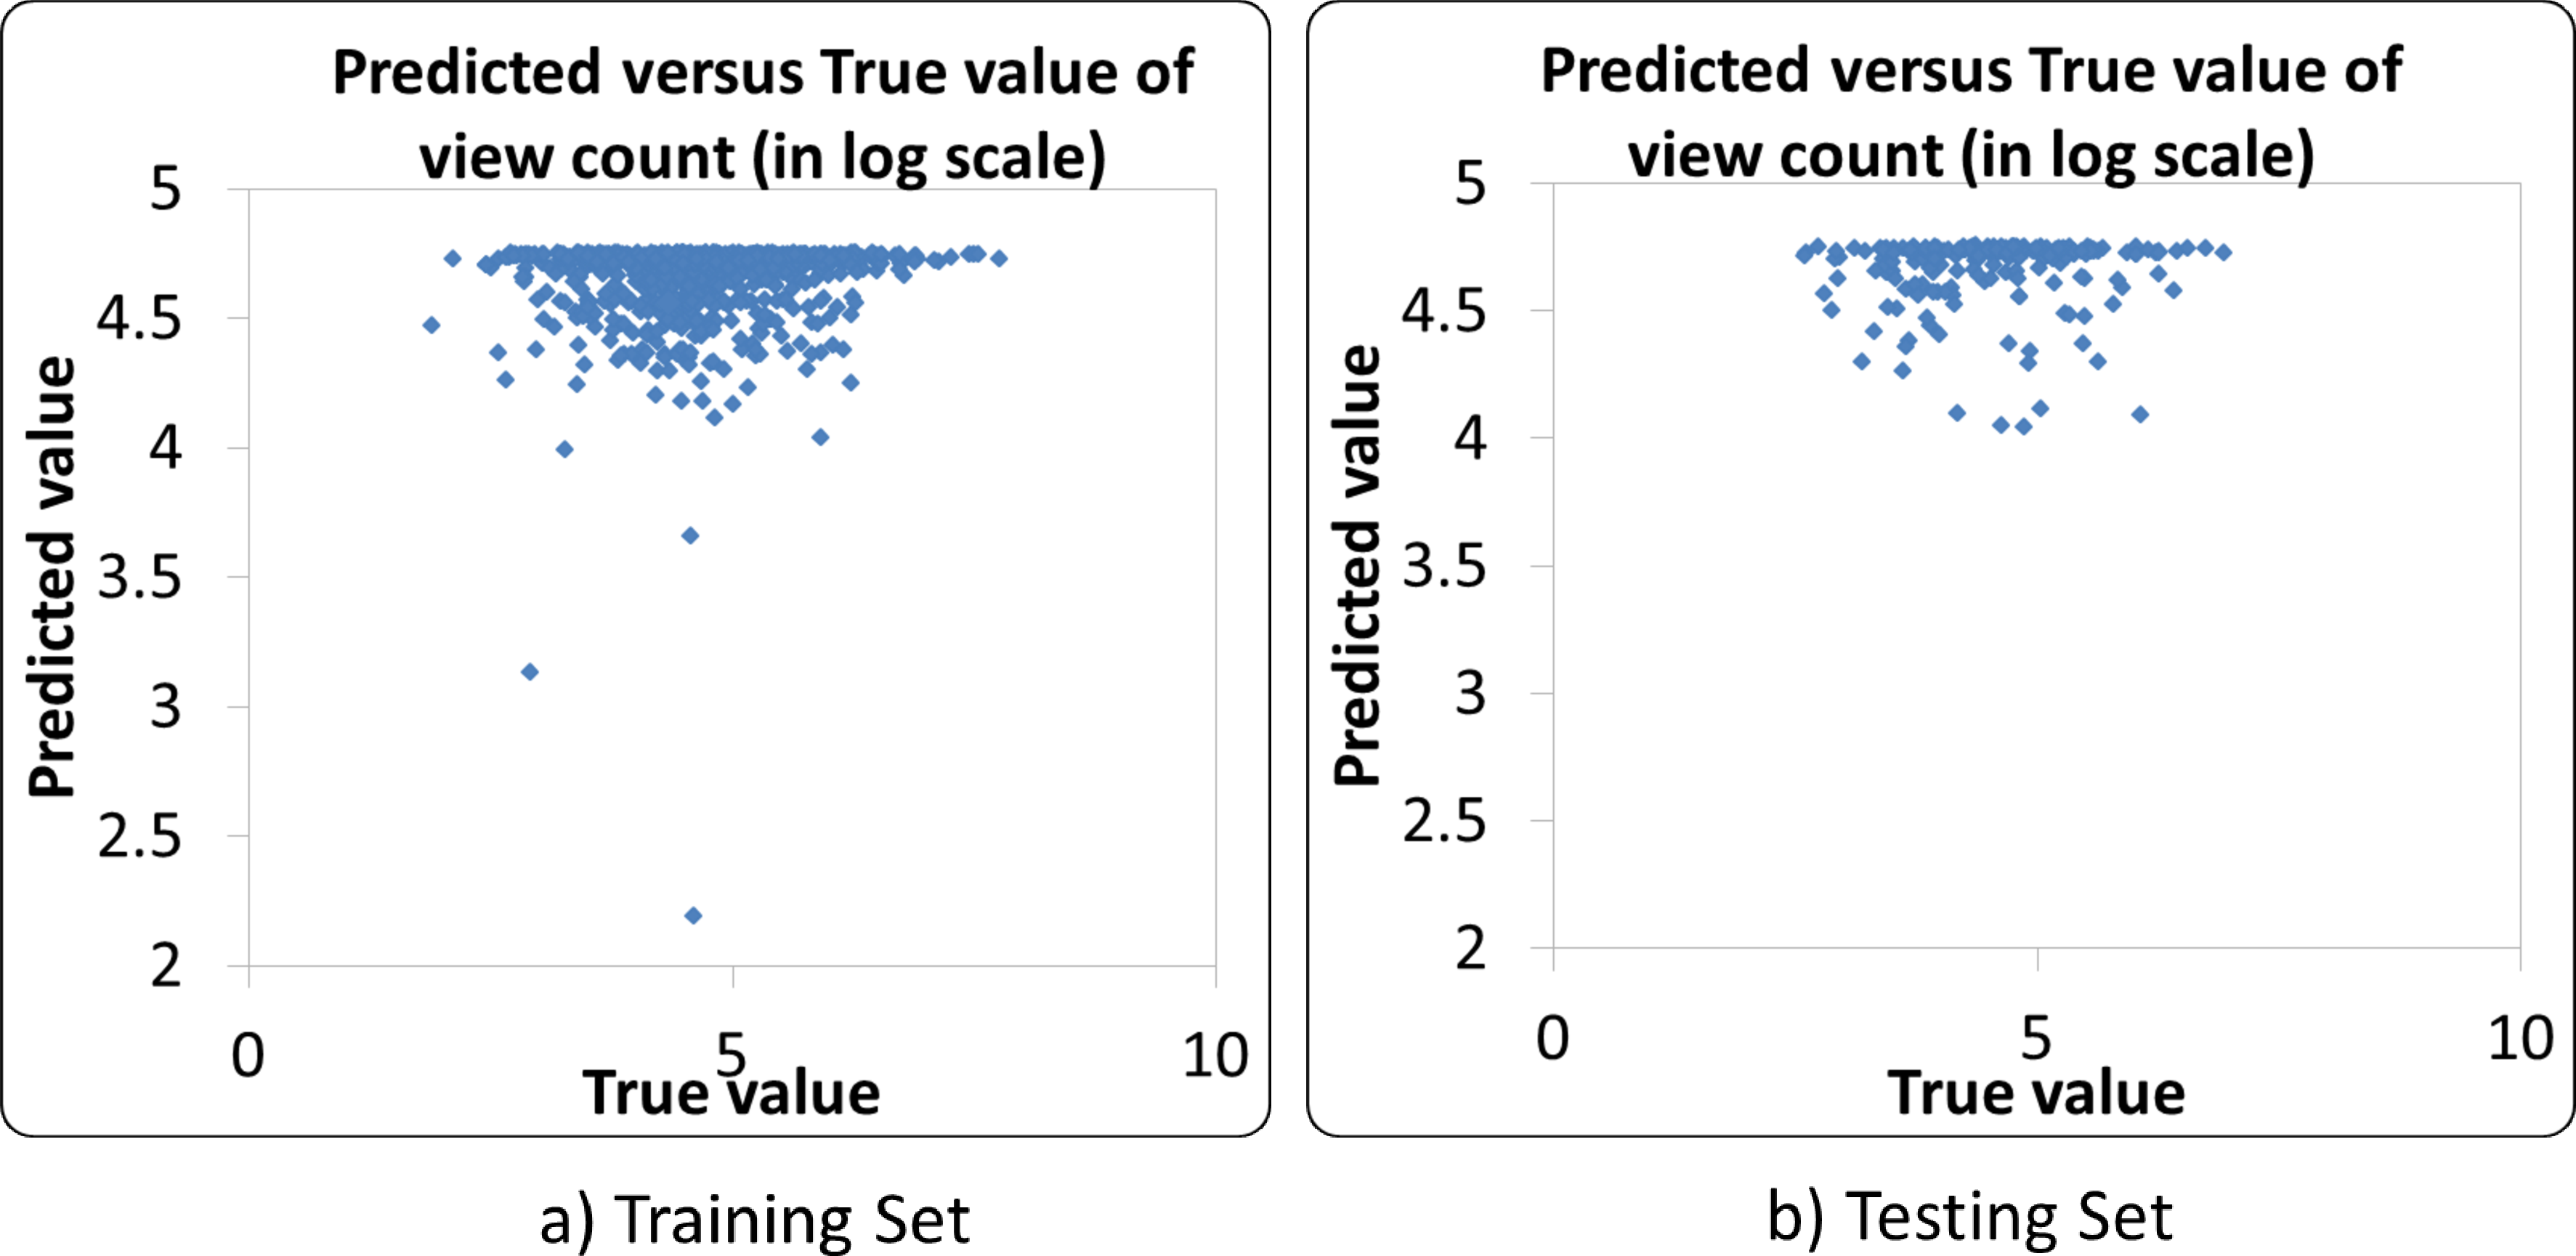
\includegraphics[width=.75\textwidth,clip]{regression.pdf}
		\end{center}
		\caption{True value vs prediction (in log-scale).}
		\label{fig:trainingTrueVsPredicted}
	\end{figure}
		
	We observe a strong tendency towards the same output value (roughly 50,000 views), which corresponds to the average number of views.  This matches the typical outcome when linear regression is inadequate: failing to match trends, the average is selected nearly always in order to minimize loss.
